\documentclass[12pt]{article}
\usepackage[utf8]{inputenc}
\usepackage{titlesec}

\usepackage{amsmath}

\usepackage{tikz}
\usepackage{caption}
\usetikzlibrary{matrix,chains,positioning,decorations.pathreplacing,arrows}

\usepackage{graphicx}
\graphicspath{ {images/} }

\usepackage{url}

\renewcommand{\figurename}{Fig.}

\titleclass{\subsubsubsection}{straight}[\subsection]
\newcounter{subsubsubsection}[subsubsection]
\renewcommand\thesubsubsubsection{\thesubsubsection.\arabic{subsubsubsection}}
\renewcommand\theparagraph{\thesubsubsubsection.\arabic{paragraph}}
\titleformat{\subsubsubsection}
  {\normalfont\normalsize\bfseries}{\thesubsubsubsection}{1em}{}
\titlespacing*{\subsubsubsection}
{0pt}{3.25ex plus 1ex minus .2ex}{1.5ex plus .2ex}

\makeatletter

\def\toclevel@subsubsubsection{4}
\def\l@subsubsubsection{\@dottedtocline{4}{7em}{4em}}

\makeatother

\setcounter{secnumdepth}{4}
\setcounter{tocdepth}{4}


\titleclass{\subsubsubsubsection}{straight}[\subsection]
\newcounter{subsubsubsubsection}[subsubsubsection]
\renewcommand\thesubsubsubsubsection{\thesubsubsubsection.\arabic{subsubsubsubsection}}
\renewcommand\theparagraph{\thesubsubsubsubsection.\arabic{paragraph}}
\titleformat{\subsubsubsubsection}
  {\normalfont\normalsize\bfseries}{\thesubsubsubsubsection}{1em}{}
\titlespacing*{\subsubsubsubsection}
{0pt}{3.25ex plus 1ex minus .2ex}{1.5ex plus .2ex}

\makeatletter

\def\toclevel@subsubsubsubsection{5}
\def\l@subsubsubsubsection{\@dottedtocline{5}{11em}{4em}}

\makeatother

\setcounter{secnumdepth}{5}
\setcounter{tocdepth}{5}

\title{}

\begin{document}

\tableofcontents

\section{Introducción}

El cerebro humano es un sistema de cálculo muy complejo, puede llevar a cabo procesamientos que a primera vista parecen sencillos, como por ejemplo, el reconocimiento de imágenes. Esta capacidad que tiene el cerebro humano para pensar, recordar y resolver problemas ha inspirado a muchos científicos a intentar imitar estos funcionamientos.\hfill \break

Los intentos de crear un ordenador que sea capaz de emular estas capacidades ha dado como resultado la aparición de las llamadas Redes Neuronales Artificales o Computación Neuronal.\hfill \break

El principal objetivo del Reconocimiento de patrones es la clasificación ya sea supervisada o no supervisada. Aplicaciones como Data Mining, Web Searching, recuperación de datos multimedia, reconocimiento de rostros, reconocimientos de caracteres escritos a mano, etc., requieren de técnicas de reconocimiento de patrones robustas y eficientes.
Las redes neuronales, por su capacidad de generalización de la información disponible y su tolerancia al ruido, constituyen una herramienta muy útil en la resolución de este tipo de problemas.\cite{patterRecognition}\hfill \break

Este documento muestra los conceptos básicos de las Redes Neuronales y su regla de aprendizaje, en particular la configuración en \textit{Perceptrón Multicapa} y el varios algoritmos de aprendizaje (Propagación hacia atrás,Métodos de segundo orden, RPROP, Algoritmos Genéticos).


\clearpage

\section{Neurona Artificial}
Uno de los retos más importantes a los que se enfrenta el ser humano de nuestra generaciónes el de la construcción de sistemas inteligentes, en su afán de conseguir este propósito aparecen las redes neuronales artificiales. Desde el punto de vista biológico las RNA son un modelo matemático acerca del funcionamiento del cerebro.\textit{"Los sencillos elementosde cálculo aritmético equivalen a las neuronas-células que procesan la información en elcerebro- y la red en general equivale a un conjunto de neuronas conectadas entre sí"} \cite{IA}\hfill \break

Para la raza humana sigue siendo un misterio el funcionamiento del cerebro humano ycomo se genera el pensamiento, sin embargo años y años de investigación han dado ideassobre el accionar del mismo. Si se quieren reproducir las acciones del cerebro humano, sedebe tener la idea de como funciona. Una explicación sencilla y clara se encuentra en \cite{IA}:

\begin{center}
\textit{"Sabemos que la neurona, o célula nerviosa, es la unidad funcional básica de los tejidos del sistema nervioso, incluido el cerebro. Las neuronas están for-madas por el cuerpo de la célula, o soma, en donde se aloja el núcleo de la célula. Del cuerpo de la célula salen ramificaciones de diversas fibras conocidas como dendritas y sale también una fibra más larga denominada axón. Las dendritas se ramifican tejiendo una tupida red alrededor de la célula, mientras el axón se extiende un buen tramo: por lo general, un centímetro (100 veces el diámetro del cuerpo de la célula) y, en casos extremos, hasta un metro. Finalmente, el axón también se ramifica en filamentos y subfilamentos mediante los que establece conexión con las dendritas y los cuerpos de las células de otras neuronas. A la unión o conexión se le conoce como sinapsis. Cada neurona establece sinapsis desde con una docena de otras neuronas hasta con cientos de miles de otras de ellas"}
\end{center}

La neurona articial se ha diseñado como una abstracción de la neurona biológica y se muestra en la Figura \ref{fig:RNA}. La figura representa  la neurona \textit{j} que recibe entradas. Sus partes son:

\clearpage

\begin{figure}[t]
\frame{
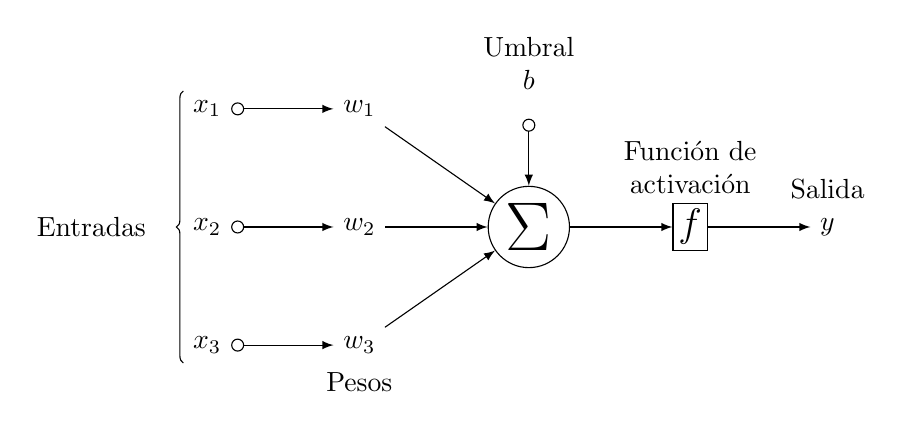
\begin{tikzpicture}[
init/.style={
  draw,
  circle,
  inner sep=2pt,
  font=\Huge,
  join = by -latex
},
squa/.style={
  draw,
  inner sep=2pt,
  font=\Large,
  join = by -latex
},
start chain=2,node distance=13mm
]
\node[on chain=2] 
  (x2) {$x_2$};
\node[on chain=2,join=by o-latex] 
  {$w_2$};
\node[on chain=2,init] (sigma) 
  {$\displaystyle\Sigma$};
\node[on chain=2,squa,label=above:{\parbox{2cm}{\centering Función de\\ activación }}]   
  {$f$};
\node[on chain=2,label=above:Salida,join=by -latex] 
  {$y$};
  
\begin{scope}[start chain=1]

\node[on chain=1] at (0,1.5cm) 
  (x1) {$x_1$};
\node[on chain=1,join=by o-latex] 
  (w1) {$w_1$};
  
\end{scope}
\begin{scope}[start chain=3]
\node[on chain=3] at (0,-1.5cm) 
  (x3) {$x_3$};
\node[on chain=3,label=below:Pesos,join=by o-latex] 
  (w3) {$w_3$};
\end{scope}

\node[label=above:\parbox{2cm}{\centering Umbral \\ $b$}] at (sigma|-w1) (wo) {};

\draw[-latex] (w1) -- (sigma);
\draw[-latex] (w3) -- (sigma);
\draw[o-latex] (wo) -- (sigma);

\draw[decorate,decoration={brace,mirror}] (x1.north west) -- node[left=10pt] {Entradas} (x3.south west);

\end{tikzpicture}
}
\centering
\caption{Representacion de una Red Neuronal Artificial.}
\label{fig:RNA}
\end{figure}

\begin{enumerate}
  \item Las \textbf{entradas} $x_i$, que son puntos por los que se reciben los datos provenientes del entorno o bien de otras neuronas. Para este caso se consideran $n$ entradas, siendo el valor de $n=3$
  \[ X = (x_1,x_2,x_3)\]
  
  \item La salida $y_i$. En una neurona biológica corresponde al axón
  \item Al igual que en una neurona biológica, la neurona artificial debe permitir establecer conexiones(sinápsis) entre las entradas(dendritas) de una neurona y la salida (axón) de otra. Esta conexión representa con una línea que tiene asociado un valor llamado \textbf{peso sináptico} $w_ji$. Nótese que el primer subíndice indice la neurona a la que llega la conexión, mientras que el segundo subíndice indica de donde viene la conexión. El peso representa el factor de importancia de la conexión en la determinación del valor de salida. El valor $w_ji$, que es un número real, se modifica durante el entrenamiento de la red neuronal y es la variable de almacenará la información que indicará que la red ha aprendido algo y por tanto que sirva para un propósito u otro.
  
  \item En la Figura \ref{fig:RNA} también se observa una entrada especial, llamada umbral, con un valor fijo que puede ser -1 o 1, y con un peso asociado llamado $w_0$. El valor del umbral se ajusta igual que cualquier otro peso durante el proceso de entrenamiento.
  
  \item Una \textbf{regla de propagación}. Para cierto valor de las entradas $x_i$ y los pesos sinápticos asociados $w_ji$, se realiza algun tipo de operación para obtener el valor del potencial \textit{post-sináptico} . Este valor es función de las entradas y los pesos. Una de las operaciones mas comunes es realizar la suma ponderada, que no es otra cosa que la sumatoria de las entradas, pero teniendo en cuenta la importancia de cada una (el peso sináptico asociado). Luego:


\[u=\sum_{i}^{\ n=3} w_{ji}x_i + w_0b\]


\item Una \textbf{función de activación}. Luego de realizar la suma ponderada, se aplica al resultado la función de activación, que se escoge de tal manera que permita obtener la forma deseada para el valor de la salida.

\begin{equation} \label{eq1}
\begin{split}
y 	&= f(u)\\
	&= f(\sum_{i}^{\ n=3} w_{ji}x_i + w_0b)\\
	&= f(W.X)\\
	&= f(W^TX)
\end{split}
\end{equation}

donde las últimas dos ecuaciones están en notación vectorial.
Es necesario especificar la función de activación $f$. Las funciones más usuales se observan en la  \ref{fig:FUNCACT}

Con estas especificaciones, se puede ahora explicar cómo funciona la neurona. Se supone en el modelo de neurona más simple, que corresponde a la función de activación escalón, tambien llamada limitador duro. En este caso, la salida puede tomar solo dos valores -1 y +1 donde la salida esta determinada por

\begin{equation}\label{eq2}
f(x) = \begin{cases}
             -1  & \text{if } u < 0 \\
             +1  & \text{if } u \ge 0
       \end{cases} \quad
\end{equation}

\clearpage

\begin{figure}[h]
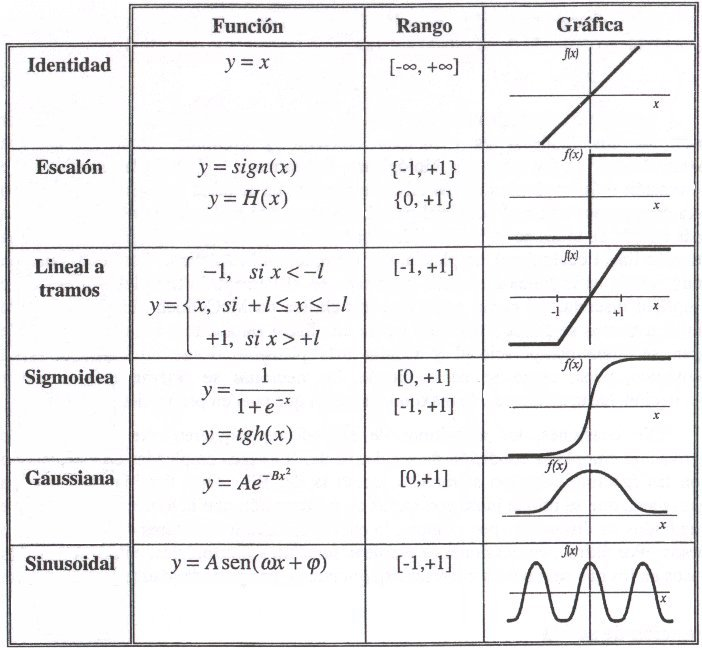
\includegraphics[width=\textwidth]{list_function}
\centering
\caption{Funciones de activación.}
\label{fig:FUNCACT}
\end{figure}

Entonces, para la función sigmoidea, se tiene que

\begin{equation} \label{eq3}
\begin{split}
y 	&= ( \frac{1}{1+e^{-u}}) \\
u	&= \sum_{i}^{\ n=3} w_{ji}x_i + w_0b
\end{split}
\end{equation}

y para el segundo caso de la función sigmoidea

\begin{equation} \label{eq3}
\begin{split}
y 	&= tanh(u) = ( \frac{e^u - e^{-u}}{e^u + e^{-u}}) \\
\end{split}
\end{equation}

La expresión de la ecuación que almacena la neurona en virtud del vector de pesos $W$ es el \textbf{modelo} que representa en mayor o menor grado el comportamiento del vector de salida y con respecto al vector de entrada $X$

\end{enumerate}

Entonces, una neurona artificial es un procesador elemental. Se encarga de procesar un vector de $n$ entradas para producir un único valor de salida $y$. El nivel de activación depende de las entradas recibidas y de los valores sinápticos. Para calcular el estado de activación se ha de calcular en primer lugar la entrada total a la célula. Este valor se cálcula como la suma de todas las entradas ponderadas por ciertos valores dados a la entrada.

\clearpage

\subsection{Redes Neuronales}
asd

\subsubsection{Redes Neuronales Supervisadas}
asd
\subsubsubsection{Redes Neuronal Perceptron Multicapa}

asd
\subsubsection{Redes Neuronales No Supervisadas}
asd


\section{Caso de Estudio}
asd
\subsection{Problema}
asd
\subsection{Justificacion}
asd
\subsection{Propuestas de Solucion}
asd
\subsubsection{Topologia}
asd
\subsubsection{Reglas}
asd
\subsubsubsection{Regla de propagación}
asd
\subsubsubsection{Regla de Activacion}
asd
\subsubsubsection{Regla de Salida}
asd
\subsubsubsection{Regla de Aprendizaje}
asd
\subsubsubsubsection{Back Propagation}
asd
\subsubsubsubsection{Segundo Orden}
asd
\subsubsubsubsection{R-PROP}
asd
\subsubsubsubsection{Algoritmos Geneticos}
asd

\subsection{Desarrollo de la solucion}
asd
\subsubsection{Herramientas}
asd
\subsubsubsection{R}
asd
\subsubsubsection{RStudio}
asd
\subsubsubsection{Package}
asd
\subsubsection{Implementacion}
asd
\subsubsubsection{Back Propagation}
asd
\subsubsubsection{Segundo Orden}
asd
\subsubsubsection{R-PROP}
asd
\subsubsubsection{Algoritmos Geneticos}
asd

\subsection{Resultados}
asd
\subsection{Conclusiones}
asd




\bibliographystyle{unsrt}
\bibliography{bibliography}

\end{document}
